% Politecnico di Milano (PoliMi) - School of Industrial and Information Engineering
%
% Copyright 2021 Politecnico di Milano, Italy. Inc. NC-BY

\documentclass[11pt,a4paper]{article} 

%------------------------------------------------------------------------------
%	REQUIRED PACKAGES AND  CONFIGURATIONS
%------------------------------------------------------------------------------
% PACKAGES FOR TITLES
\usepackage{titlesec}
\usepackage{color}

% PACKAGES FOR LANGUAGE AND FONT
\usepackage[utf8]{inputenc}
\usepackage[english]{babel}
\usepackage[T1]{fontenc} % Font encoding

% PACKAGES FOR IMAGES
\usepackage{graphicx}
\graphicspath{{Images/}}
\usepackage{eso-pic} % For the background picture on the title page
\usepackage{subfig} % Numbered and caption subfigures using \subfloat
\usepackage{caption} % Coloured captions
\usepackage{transparent}

% STANDARD MATH PACKAGES
\usepackage{amsmath}
\usepackage{amsthm}
\usepackage{bm}
\usepackage[overload]{empheq}  % For braced-style systems of equations

% PACKAGES FOR TABLES
\usepackage{tabularx}
\usepackage{longtable} % tables that can span several pages
\usepackage{colortbl}
\usepackage{array}
\usepackage{rotating}
\usepackage{afterpage}

% PACKAGES FOR ALGORITHMS (PSEUDO-CODE)
\usepackage{algorithm}
\usepackage{algorithmic}

% PACKAGES FOR REFERENCES & BIBLIOGRAPHY
\usepackage[colorlinks=true,linkcolor=black,anchorcolor=black,citecolor=black,filecolor=black,menucolor=black,runcolor=black,urlcolor=black]{hyperref} % Adds clickable links at references
\usepackage{cleveref}
\usepackage[sort&compress]{natbib} % Square brackets, citing references with numbers, citations sorted by appearance in the text and compressed
\bibliographystyle{abbrvnat} % You may use a different style adapted to your field
\setcitestyle{authoryear, square}

% PACKAGES FOR THE APPENDIX
\usepackage{appendix}

% PACKAGES FOR ITEMIZE & ENUMERATES 
\usepackage{enumitem}

% OTHER PACKAGES
\usepackage{amsthm,thmtools,xcolor} % Coloured "Theorem"
\usepackage{comment} % Comment part of code
\usepackage{fancyhdr} % Fancy headers and footers
\usepackage{lipsum} % Insert dummy text
\usepackage{tcolorbox} % Create coloured boxes (e.g. the one for the key-words)

%-------------------------------------------------------------------------
%	NEW COMMANDS DEFINED
%-------------------------------------------------------------------------
% EXAMPLES OF NEW COMMANDS -> here you see how to define new commands
\newcommand{\bea}{\begin{eqnarray}} % Shortcut for equation arrays
\newcommand{\eea}{\end{eqnarray}}
\newcommand{\e}[1]{\times 10^{#1}}  % Powers of 10 notation
\newcommand{\mathbbm}[1]{\text{\usefont{U}{bbm}{m}{n}#1}} % From mathbbm.sty
\newcommand{\pdev}[2]{\frac{\partial#1}{\partial#2}}
% NB: you can also override some existing commands with the keyword \renewcommand

%----------------------------------------------------------------------------
%	ADD YOUR PACKAGES (be careful of package interaction)
%----------------------------------------------------------------------------


%----------------------------------------------------------------------------
%	ADD YOUR DEFINITIONS AND COMMANDS (be careful of existing commands)
%----------------------------------------------------------------------------


% Do not change Configuration_files/config.tex file unless you really know what you are doing. 
% This file ends the configuration procedures (e.g. customizing commands, definition of new commands)
% Configuration package
\usepackage[bottom=2.0cm,top=2.0cm,left=2.0cm,right=2.0cm]{geometry}
\raggedbottom 

% Create color bluePoli (-> manuale grafica coordinata:  https://www.polimi.it/fileadmin/user_upload/il_Politecnico/grafica-coordinata/2015_05_11_46xy_manuale_grafica_coordinata.pdf)
\definecolor{bluePoli}{cmyk}{0.4,0.1,0,0.4}

% Custom theorem environments
\declaretheoremstyle[
  headfont=\color{bluePoli}\normalfont\bfseries,
  bodyfont=\color{black}\normalfont\itshape,
]{colored}

\captionsetup[figure]{labelfont={color=bluePoli}} % Set colour of the captions
\captionsetup[table]{labelfont={color=bluePoli}} % Set colour of the captions
\captionsetup[algorithm]{labelfont={color=bluePoli}} % Set colour of the captions

\theoremstyle{colored}
\newtheorem{theorem}{Theorem}[section]
\newtheorem{proposition}{Proposition}[section]

% Enhances the features of the standard "table" and "tabular" environments.
\newcommand\T{\rule{0pt}{2.6ex}}
\newcommand\B{\rule[-1.2ex]{0pt}{0pt}}

% Algorithm description
\newcounter{algsubstate}
\renewcommand{\thealgsubstate}{\alph{algsubstate}}
\newenvironment{algsubstates}{
    \setcounter{algsubstate}{0}%
    \renewcommand{\STATE}{%
    \stepcounter{algsubstate}%
    \Statex {\small\thealgsubstate:}\space}
    }{}
    
% Custom theorem environment
\newcolumntype{L}[1]{>{\raggedright\let\newline\\\arraybackslash\hspace{0pt}}m{#1}}
\newcolumntype{C}[1]{>{\centering\let\newline\\\arraybackslash\hspace{0pt}}m{#1}}
\newcolumntype{R}[1]{>{\raggedleft\let\newline\\\arraybackslash\hspace{0pt}}m{#1}}

% Custom itemize environment
\setlist[itemize,1]{label=$\bullet$}
\setlist[itemize,2]{label=$\circ$}
\setlist[itemize,3]{label=$-$}
\setlist{nosep}

% Create command for background pic
\newcommand\BackgroundPic{% Adding background picture
	\put(237,365){
	    \parbox[b][\paperheight]{\paperwidth}{%
	    \vfill
		\centering
		\transparent{0.4}
		
\includegraphics[width=0.44\paperwidth]{raggiera_polimi.eps}%
		\vfill}
		}
}

% Set indentation
\setlength\parindent{0pt}

% Custom title commands
\titleformat{\section}
{\color{bluePoli}\normalfont\Large\bfseries}
{\color{bluePoli}\thesection.}{1em}{}
\titlespacing*{\section}
{0pt}{3.3ex}{3.3ex}

\titleformat{\subsection}
{\color{bluePoli}\normalfont\large\bfseries}
{\color{bluePoli}\thesubsection.}{1em}{}
\titlespacing*{\subsection}
{0pt}{3.3ex}{3.3ex}

% Custom headers and footers
\pagestyle{fancy}
\fancyhf{}
      
\fancyfoot{}
\fancyfoot[C]{\thepage} % page
\renewcommand{\headrulewidth}{0mm} % headrule width
\renewcommand{\footrulewidth}{0mm} % footrule width

\makeatletter
\patchcmd{\headrule}{\hrule}{\color{black}\hrule}{}{} % headrule
\patchcmd{\footrule}{\hrule}{\color{black}\hrule}{}{} % footrule
\makeatother


% Insert here the info that will be displayed into your Title page 
% -> title of your work
\renewcommand{\title}{BUMP - BUbble column Multiphase Project}
% -> author name and surname
\renewcommand{\author}{Stefano Passoni, Martina Di Gennaro, Riccardo Giordani}
% -> abstract (only in English)
\renewcommand{\abstract}{}

% -> key-words (only in English)
\newcommand{\keywords}{here, the keywords, of your thesis}

\newcommand{\thead}[2][.95in]{%
  \vbox{\hsize#1\baselineskip11pt\centering\vspace*{3pt}#2\par}}

%-------------------------------------------------------------------------
%	BEGIN OF YOUR DOCUMENT
%-------------------------------------------------------------------------
\begin{document}

%-----------------------------------------------------------------------------
% TITLE PAGE
%-----------------------------------------------------------------------------
% Do not change Configuration_files/TitlePage.tex (Modify it IF AND ONLY IF you need to add or delete the Co-advisors)
% This file creates the Title Page of the document
% DO NOT REMOVE SPACES BETWEEN LINES!

\AddToShipoutPicture*{\BackgroundPic}

\hspace{-0.6cm}
\includegraphics[width=0.6\textwidth]{logo_polimi_ing_indinf.eps}

\vspace{-1mm}
\Large{\textbf{\color{bluePoli}{\title}}}\\

\vspace{-0.2cm}
\large{\textbf{\author}}

\small \normalfont

\vspace{11pt}

\centerline{\rule{1.0\textwidth}{0.4pt}}

%\begin{center}
%\begin{minipage}{.90 \textwidth}
%\noindent \textbf{\color{bluePoli} Abstract:} {\abstract}
%\end{minipage}
%\end{center}
\tableofcontents
\vspace{11pt}
\centerline{\rule{1.0\textwidth}{0.4pt}}
\vspace{15pt}

%\begin{tcolorbox}[arc=0pt, boxrule=0pt, colback=bluePoli!60, width=\textwidth, colupper=white]
  %  \textbf{Key-words:} Bubble column, Homogeneous flow regime, Computational fluid dynamics, Validation,
%\end{tcolorbox}

\vspace{12pt}




\section{Introduction}
\label{sec:1}
Bubble columns are multiphase reactors where the dispersed phase (gas) is introduced into a stationary or flowing liquid (continuous phase) and provide a good experimental setup to study the turbulent phenomena in dense bubbly flows. The functioning is apparently simple, as the ascending gas-phase creates a buoyancy-driven flow inducing the recirculation of the liquid phase. The local and the global fluid dynamic properties are related to the prevailing flow regime which may be homogeneous (bubbly flow condition at low superficial gas velocity, tipically $U_G<$ 0.03 $m/s$) or heterogeneous (churn-turbulent flow condition, $U_G>$ 0.1 $m/s$, $\alpha_G \geq$ 0.3). The homogeneous flow regime can be classified into the \textit{mono-dispersed homogeneous} flow regime, characterized by a mono-dispersed bubble size distribution (BSD), and the \textit{pseudo-homogeneous} flow regime, characterized by a poly-dispersed BSD. The distinction between mono-dispersed and poly-dispersed BSDs is based upon the change in the sign of the lift force coefficient. \\
Numerous industrial designs have been based on empirical correlations, but such approaches remain somewhat limited when increasing the reactor performance is sought. To improve the description of the physical phenomenon occurring in bubble columns a promising numerical method is the Computational Fluid Dynamics (CFD). CFD helps to understand the complex two-phase fluid dynamics in the bubble column through details of mean flows (fields of three components of mean velocities and mean gas hold-up), interphase rates of mass, energy and momentum transfer and turbulence parameters (such as turbulent kinetic energy, energy dissipation rate, Reynolds stresses, etc.). \\
In the present work, bubble column is numerically simulated by using the open source CFD tool OpenFOAM []. More in detail, the objective of the present work is the validation of the already existing \textit{multiphaseEulerFoam} solver working for the case of \textit{mono-dispersed homogeneous} bubble column. For the case study we have considered a multiphase mixture of air and water without taking into account the heat transfer phenomena. \\
The \textit{multiphaseEulerFoam} is used for simulation of incompressible multiphase flows in vertical pipelines. This model combines the Eulerian-Eulerian (two-fluid).
\\ 
The structure of the report is as follows. In Section 2, the experimental benchmark taken as reference is illustrated. In Section 3,



\section{Experimental Benchmark}
\label{sec:2}
The  experimental benchmark taken as reference for the validation comes from the literature, in particular from the study of Krepper et al. []. The experimental setup consists of three rectangular channels 20cm$^2$ in cross-section (0.1 × 0.02 $m$) bolted together at the flanges resulting in a bubble column of 1-meter height (fig 1.). The test facility is initially filled with water up to a specified (..) height. In the bottom of the test section is present a rectangular porous stone adopted as gas sparger 0.02$m$ wide, 0.01$m$ depth and 0.01$m$ height.This sparger produced a \textit{mono-dispersed homogeneous} bubble size distribution with a bubble diameter of 3-5 $mm$. The superficial gas flow rate, $U_G$, is varied between three different value, 0.006 $m/s$, 0.008 $m/s$ and 0.010 $m/s$, in the \textit{mono-dispersed homogenous} flow regime. The superficial velocity is calculated from the measured volume flow rates using: 
\begin{equation}
    U_G=\frac{Q_G}{A_{CS}}
\end{equation}
where $Q_G$ is the measured volume flow rate of the gas and $A_{CS}$ is the cross-sectional area of the test section. The column operates in the dispersed bubble bubbly regime, characterized by the absence of bubble coalescence or breakup, for the superficial gas velocities adopted in this work. For each superficial gas velocity the volume average void fraction, $\alpha_V$, also known as \textit{gas holdup}, can be calculated using: 
\begin{equation}
    \alpha_V=\frac{h_{final}-h_{initial}}{h_{final}}
\end{equation}
where $h_{final}$ is the heigth of the liquid column after the column has been aerated and $h_{initial}$ is the stationary height of the liquid column before aeration. The experimental data consist of wire-mesh local void fraction measurements performed at two different axial heights y = 0.08 $m$ and y = 0.63 $m$ above the gas sparger). The wire mesh sensor is placed in the cross-section by bolting it to two flanged rectangular channels. The wire-mesh sensor data was recorded at a frequency of 2500 Hz for a time period of 60 s. 

%-----------------------------------------------------------------------------
% NUMERICAL SETUP
%-----------------------------------------------------------------------------
\section{Numerical Setup}
\label{sec:numsetup}
In this section all the details related to the numerical setup will be presented and discussed.




\subsection{Domain and Mesh}
\label{sub:domain}
The numerical domain has been modeled and meshed with the utility \texttt{blockMesh}.






\subsection{Boundary Conditions}
\label{sub:bc}
The list of boundary conditions applied to the domain is summarized in table XX. At the inlet, three different mass flow rates were applied corresponding to the gas superficial velocities studied, respectively 6, 8 and 10 mm/s. These superficial velocities are an experimental input and were calculated as the volumetric flow rate of gas injected in the column divided by its volume. In OpenFOAM, this boundary condition was applied



\subsection{Solver}
\label{sub:solver}




\subsection{Multiphase Forces}
\label{sub:forces}









%-----------------------------------------------------------------------------
% RESULTS AND DISCUSSION
%-----------------------------------------------------------------------------
\section{Results and Discussion}
\label{sec:results}



\subsection{CFD methodology}
\label{sub:methodology}


%\afterpage{
%\clearpage
\begin{sidewaystable}
    \centering 
    \begin{tabular}{|p{3em} c c c c c c c c|}
    \hline
    \rowcolor{bluePoli!40}
     & \thead{\textbf{$J_{in} [mm/s]$}} & \thead{\textbf{Mesh}} & \thead{\textbf{Time step}} &  \thead{\textbf{Turbulence model}}  & \thead{\textbf{Drag model}}  & \thead{\textbf{Lift model}} &  \thead{\textbf{Turbulent dispersion model}} & \thead{\textbf{Wall lubrication model}}\T\B \\
    \hline \hline
    \textbf{run001} & 10 & A & 0.005  & kOmegaSSTSato   & IshiiZuber & Tomiyama & None & None \T\B \\
    \textbf{run002} & 10 & B & 0.005  & kOmegaSSTSato   & IshiiZuber & Tomiyama & None & None \T\B \\
    \textbf{run003} & 10 & C & 0.005  & kOmegaSSTSato   & IshiiZuber & Tomiyama & None & None \T\B \\
    \textbf{run004} & 10 & D & 0.005  & kOmegaSSTSato   & IshiiZuber & Tomiyama & None & None \T\B \\
    \textbf{run005} & 10 & A & 0.010  & kOmegaSSTSato   & IshiiZuber & Tomiyama & None & None \T\B \\
    \textbf{run006} & 10 & A & 0.0025 & kOmegaSSTSato   & IshiiZuber & Tomiyama & None & None \T\B \\
    \textbf{run007} & 10 & A & 0.005  & LaheyKEpsilon   & IshiiZuber & Tomiyama & None & None \T\B \\
    \textbf{run008} & 10 & A & 0.005  & mixtureKEpsilon & IshiiZuber & Tomiyama & None & None \T\B \\
    \textbf{run009} & 10 & A & 0.005  & kOmegaSSTSato   & IshiiZuber & None     & None & None \T\B \\
    \textbf{run010} & 10 & A & 0.005  & kOmegaSSTSato   & IshiiZuber & Moraga   & None & None \T\B \\
    \textbf{run011} & 10 & A & 0.005  & kOmegaSSTSato   & IshiiZuber & Tomiyama & Burns & None \T\B \\
    \textbf{run012} & 10 & A & 0.005  & kOmegaSSTSato   & IshiiZuber & Tomiyama & LopezDeBertodanonone & None \T\B \\
    \textbf{run013} & 10 & A & 0.005  & kOmegaSSTSato   & IshiiZuber & Tomiyama & Burns & Antal \T\B \\
    \textbf{run014} & 10 & A & 0.005  & kOmegaSSTSato   & IshiiZuber & Tomiyama & Burns & Frank \T\B \\
    \textbf{run015} & 8  & A & 0.005  & kOmegaSSTSato   & IshiiZuber & Tomiyama & Burns & Antal \T\B \\
    \textbf{run016} & 6  & A & 0.005  & kOmegaSSTSato   & IshiiZuber & Tomiyama & Burns & Antal \T\B \\
    \hline
    \end{tabular}
    \\[10pt]
    \caption{Runs performed}
    \label{table:example}
\end{sidewaystable}
%}

\subsection{Mesh sensitivity}
\label{sub:mesh_sensitivity}

\begin{table}[H]
    \centering 
    \begin{tabular}{|p{5em} c c c c |}
    \hline
    \rowcolor{bluePoli!40}
    & & \textbf{$N_x$} & \textbf{$N_y$} & \textbf{$N_z$} \T\B \\
    \hline \hline
    \textbf{run001} & \textbf{Mesh A} & 20 & 200 & 4 \T\B \\
    \textbf{run002} &\textbf{Mesh B} & 20 & 200 & 8 \T\B \\
    \textbf{run003} &\textbf{Mesh C} & 40 & 200 & 8 \T\B \\
    \textbf{run004} &\textbf{Mesh D} & 40 & 400 & 8 \T\B \\
    \hline
    \end{tabular}
    \\[10pt]
    \caption{Meshes}
    \label{table:meshes}
\end{table}

\begin{figure}[H]
    \centering
    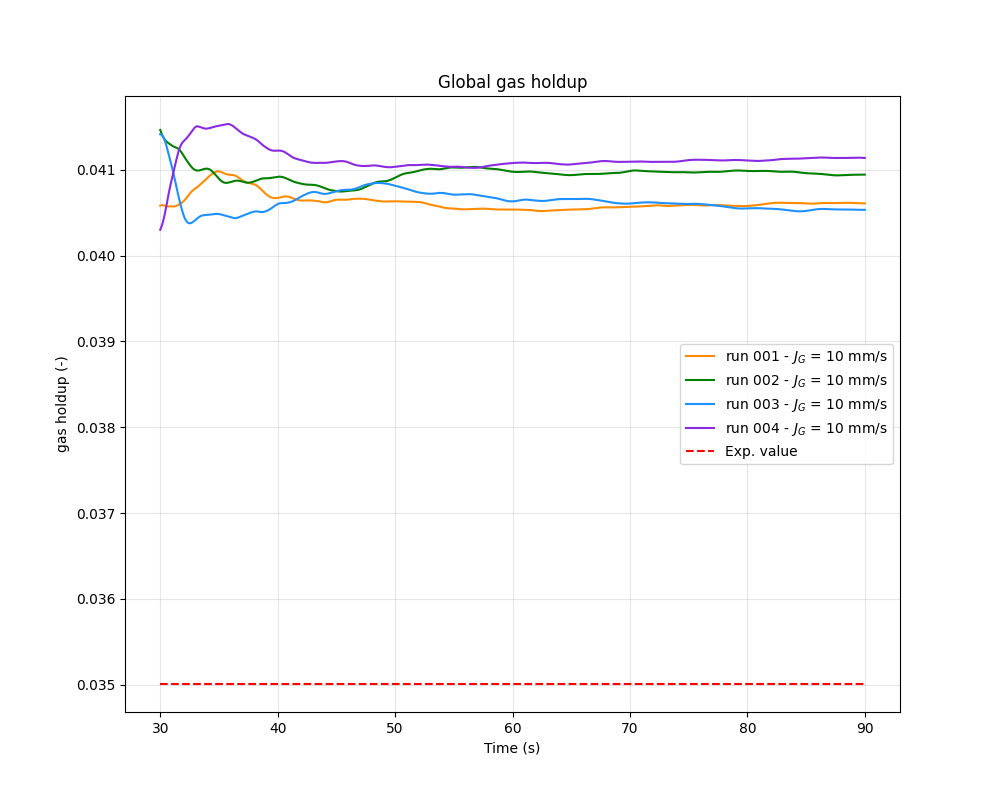
\includegraphics[width=0.5\textwidth]{Images/graphs/mesh/holdUp10.png}
    \caption{Averaged holdup for different meshes}
    \label{fig:holdup_mesh}
\end{figure}

\begin{figure}[H]
    \centering
    \subfloat[h = 8 cm]{
        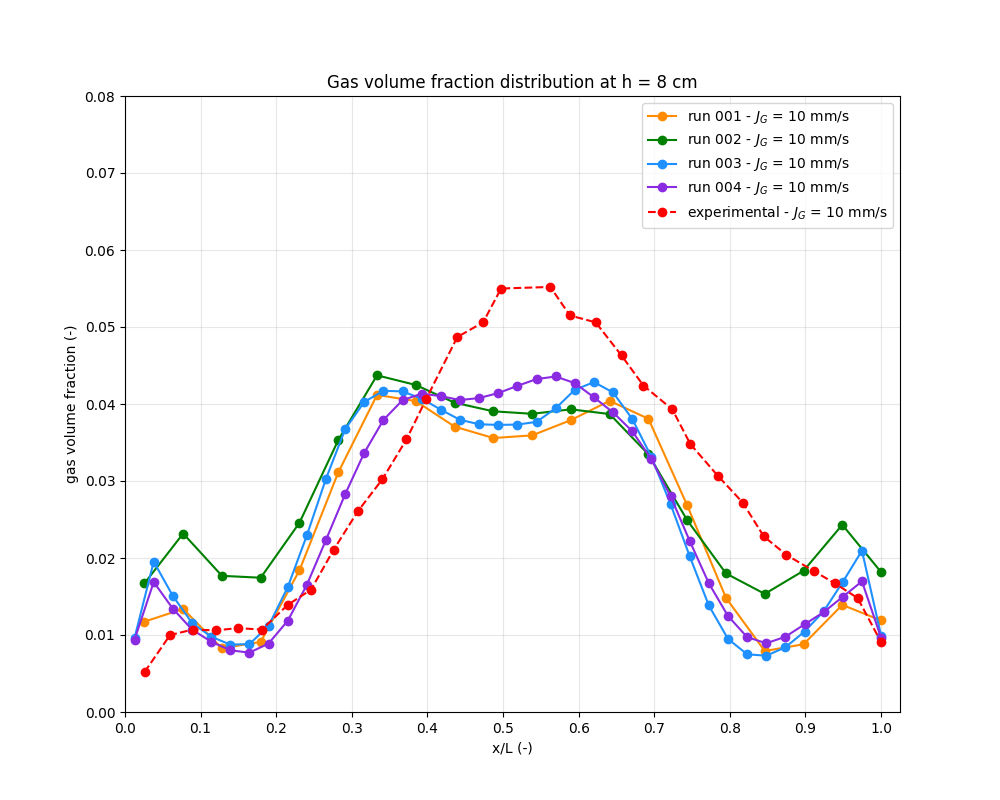
\includegraphics[scale=0.35]{Images/graphs/mesh/surfacesJ10h8.png}
    }
    \subfloat[h = 63 cm]{
        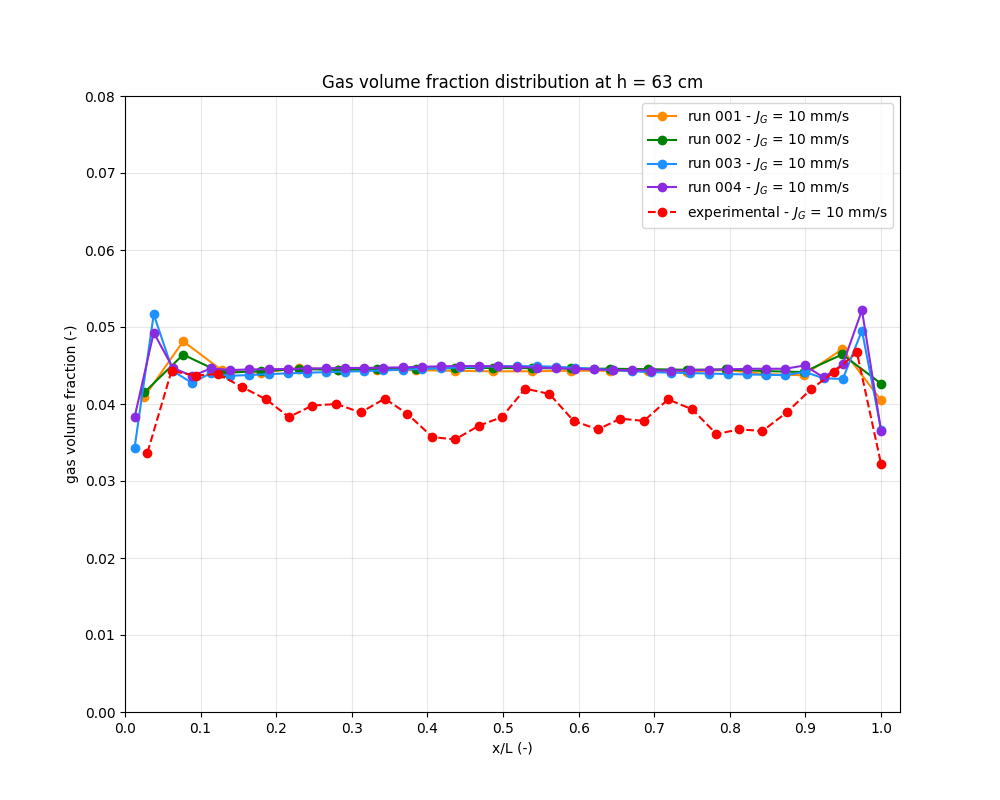
\includegraphics[scale=0.35]{Images/graphs/mesh/surfacesJ10h63.png}
    }
    \caption[]{Gas volume fraction horizontal distribution at different heights for different meshes}
    \label{fig:alpha_mesh}
\end{figure}

\subsection{Time sensitivity}
\label{sub:time_sensitivity}

\begin{table}[H]
    \centering 
    \begin{tabular}{|p{8em} c |}
    \hline
    \rowcolor{bluePoli!40}
     & \textbf{$\Delta t$} \T\B \\
    \hline \hline
    \textbf{run006} & 0.0025 \T\B \\
    \textbf{run001} & 0.005 \T\B \\
    \textbf{run005} & 0.010 \T\B \\
    \hline
    \end{tabular}
    \\[10pt]
    \caption{Time steps}
    \label{table:time_steps}
\end{table}

\begin{figure}[H]
    \centering
    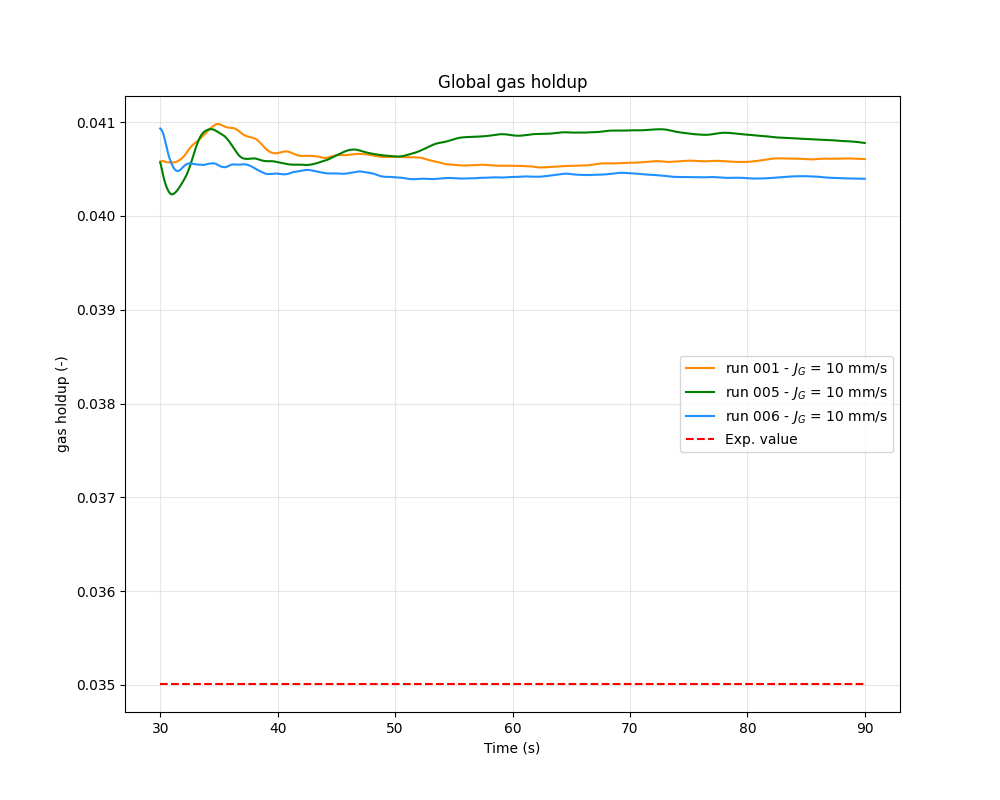
\includegraphics[width=0.5\textwidth]{Images/graphs/time/holdUp10.png}
    \caption{Averaged holdup for different time steps}
    \label{fig:holdup_time}
\end{figure}

\begin{figure}[H]
    \centering
    \subfloat[h = 8 cm]{
        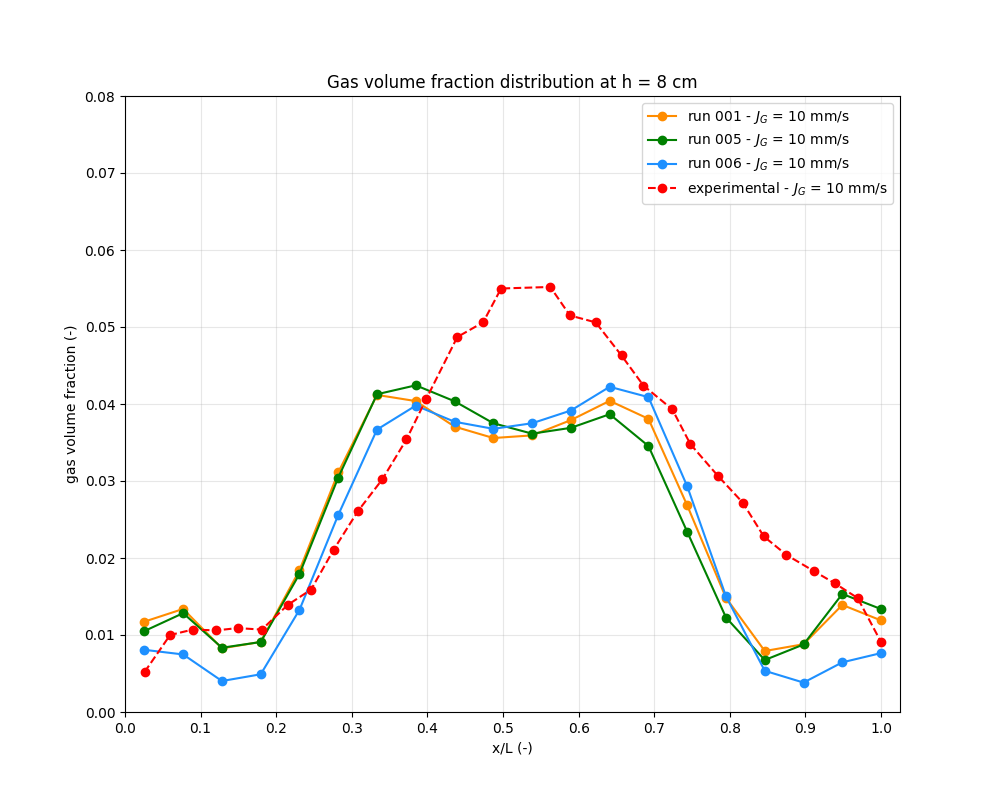
\includegraphics[scale=0.35]{Images/graphs/time/surfacesJ10h8.png}
    }
    \subfloat[h = 63 cm]{
        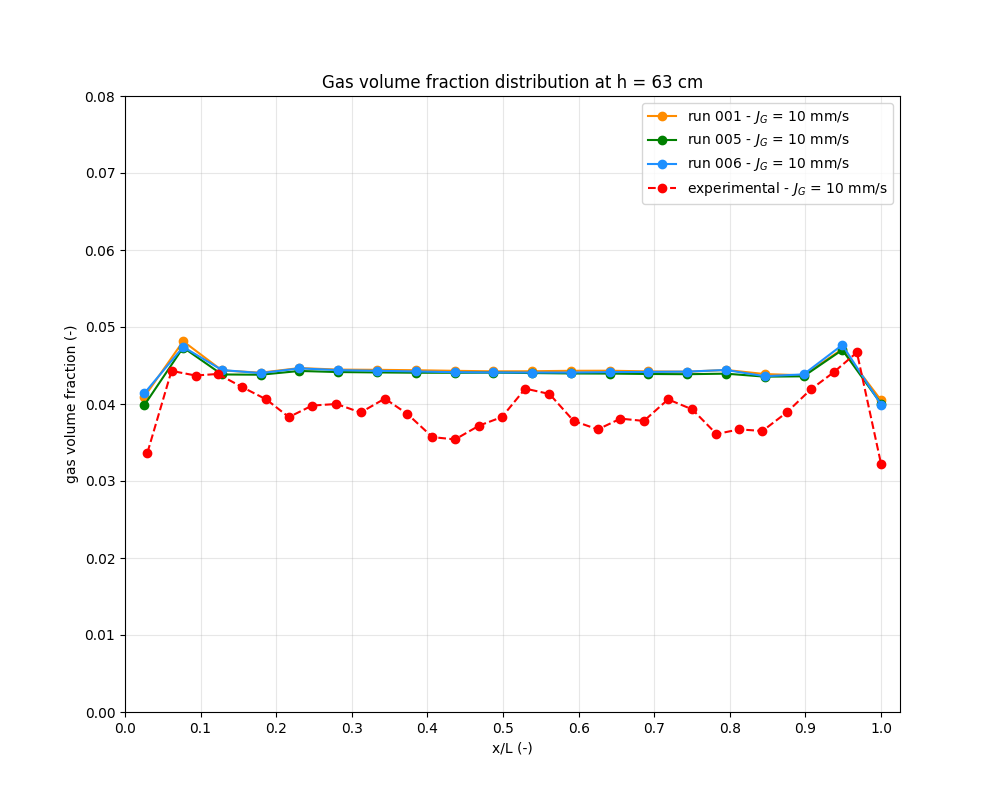
\includegraphics[scale=0.35]{Images/graphs/time/surfacesJ10h63.png}
    }
    \caption[]{Gas volume fraction horizontal distribution at different heights for different time steps}
    \label{fig:alpha_time}
\end{figure}

\subsection{Turbulence models}
\label{sub:turbulence_models}

\subsubsection{\boldmath$k-\omega$ SST Sato}
The \textit{$k-\omega$ SST Sato} model \citep{SSTSato} has originally developed to tackle the problem of heat transfer for boundary layer flows. It combines eddy-viscosity models for the momentum equations and eddy-diffusivity model for heat transer. \\
The idea behind SST model is to combine the best elements of the $k-\epsilon$ model and the $k-\omega$ model with the help of a blending function. Indeed, the $k-\epsilon$ model presents deficiencies near the wall, where fine meshes and specific near-wall treatments are required. Whereas, the $k-\omega$ model is strongly dependent of the solution to free stream values of $\omega$ outside the boundary layer.

\begin{flalign}
   \hspace{2cm}	&\frac{\partial \rho k}{\partial t} + \frac{\partial \rho U_j k}{\partial x_j} 	= \tilde{P_k} - \beta^\star \rho \omega k + \frac{\partial}{\partial x_j}			\left(\Gamma_k \frac{\partial k}{\partial x_j}\right) \label{eq:k-equation_kOmegaSSTSato} & \\
   	&\frac{\partial \rho \omega}{\partial t} + \frac{\partial \rho U_j \omega}{\partial x_j} = \frac{\gamma}{\nu_t}P_k - \beta \rho \omega^2 + \frac{\partial}{\partial x_j}\left(\Gamma_\omega \frac{\partial \omega}{\partial x_j}\right) + (1-F_1)2\rho\sigma_{\omega 2}\frac{1}{\omega}\frac{\partial k}{\partial x_j}\frac{\partial \omega}{\partial x_j} \label{eq:omega-equation_kOmegaSSTSato}&
\end{flalign}
with
\begin{flalign}
   \hspace{2cm}	& \Gamma_k = \mu + \frac{\mu_t}{\sigma_k}, \hspace{0.1cm} \Gamma_\omega = \mu + \frac{\mu_t}{\sigma_\omega}, \hspace{0.1cm} P_k = \tau_{ij}\frac{\partial U_i}{\partial x_j}, \hspace{0.1cm} \tilde{P_k} = \min(P_k;c_l\epsilon), \hspace{0.1cm} \mu_t = \rho\frac{a_1k}{\max(a_1\omega; S \cdot F_2)} &
\end{flalign}
The coefficients, $\phi$ of the model are function of $F_1$: $\phi = F_1 \phi_1 + (1-F_1)\phi_2$, where $\phi_1$ and $\phi_2$ stand for the coefficients fo the $k-\omega$ and the $k-\epsilon$ model rispectively:
\begin{flalign}
   \hspace{2cm}	& \sigma_{k1}=1.176, \hspace{0.1cm} \sigma_{\omega 1}=2.000, \hspace{0.1cm} \kappa = 0.41, \hspace{0.1cm} \gamma_1 = 0.5532, \hspace{0.1cm} \beta_1 = 0.0750, \hspace{0.1cm} \beta^\star = 0.09, \hspace{0.1cm} c_1 = 10 & \\
   & \sigma_{k2}=1.00, \hspace{0.1cm} \sigma_{\omega 2}=1.168, \hspace{0.1cm} \kappa = 0.41, \hspace{0.1cm} \gamma_2 = 0.4403, \hspace{0.1cm} \beta_2 = 0.0828, \hspace{0.1cm} \beta^\star = 0.09&
\end{flalign}
with
\begin{flalign}
   \hspace{2cm}	& F_1 = \tanh &
\end{flalign}
Here, the absolute value of the strain rate, S, is used in the definition of the eddy viscosity instead of the vorticity in order to increase the generality of the method beyond aerodynamic applications.\\
The turbulent heat flux vector is modelled with the help of a turbulent diffusivity:





















\subsubsection{Lahey $k-Epsilon$}

\subsubsection{Mixture $k-Epsilon$}

\begin{table}[H]
    \centering 
    \begin{tabular}{|p{8em} c |}
    \hline
    \rowcolor{bluePoli!40}
    & \textbf{Turbulence model} \T\B \\
    \hline \hline
    \textbf{run001} & kOmegaSSTSato \T\B \\
    \textbf{run007} & LaheyKEpsilon \T\B \\
    \textbf{run008} & mixtureKEpsilon \T\B \\
    \hline
    \end{tabular}
    \\[10pt]
    \caption{Turbulence models}
    \label{table:turbulence_models}
\end{table}

\begin{figure}[H]
    \centering
    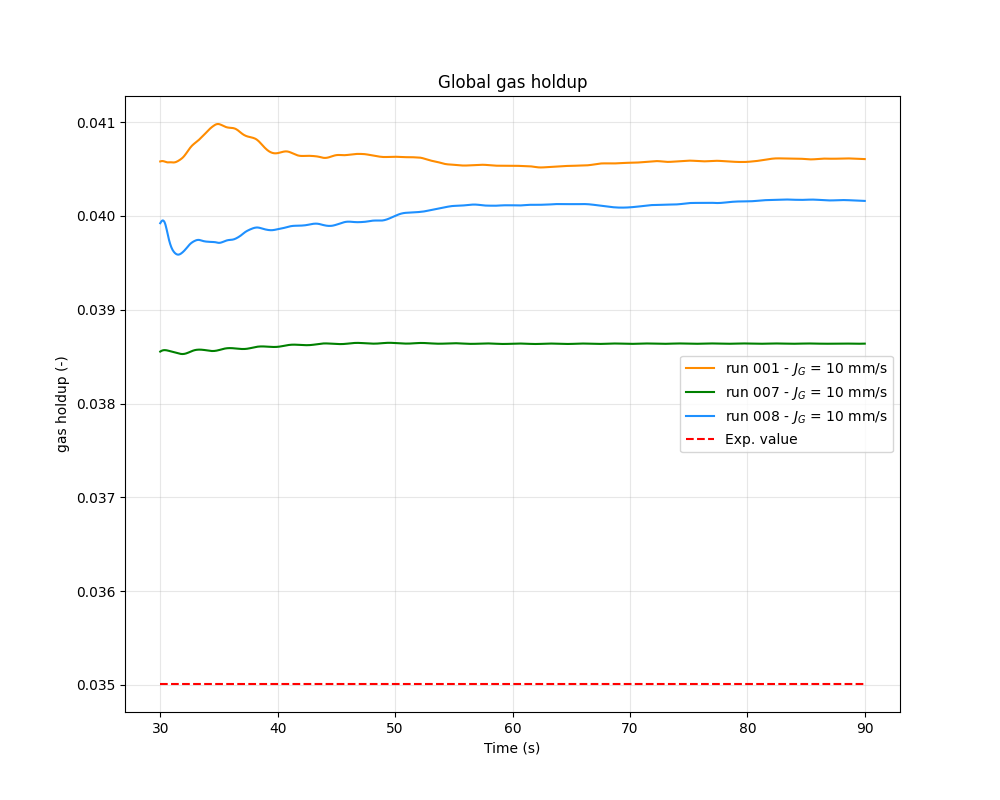
\includegraphics[width=0.5\textwidth]{Images/graphs/turbmodel/holdUp10.png}
    \caption{Averaged holdup for different turbulence models}
    \label{fig:holdup_turbmodel}
\end{figure}

\begin{figure}[H]
    \centering
    \subfloat[h = 8 cm]{
        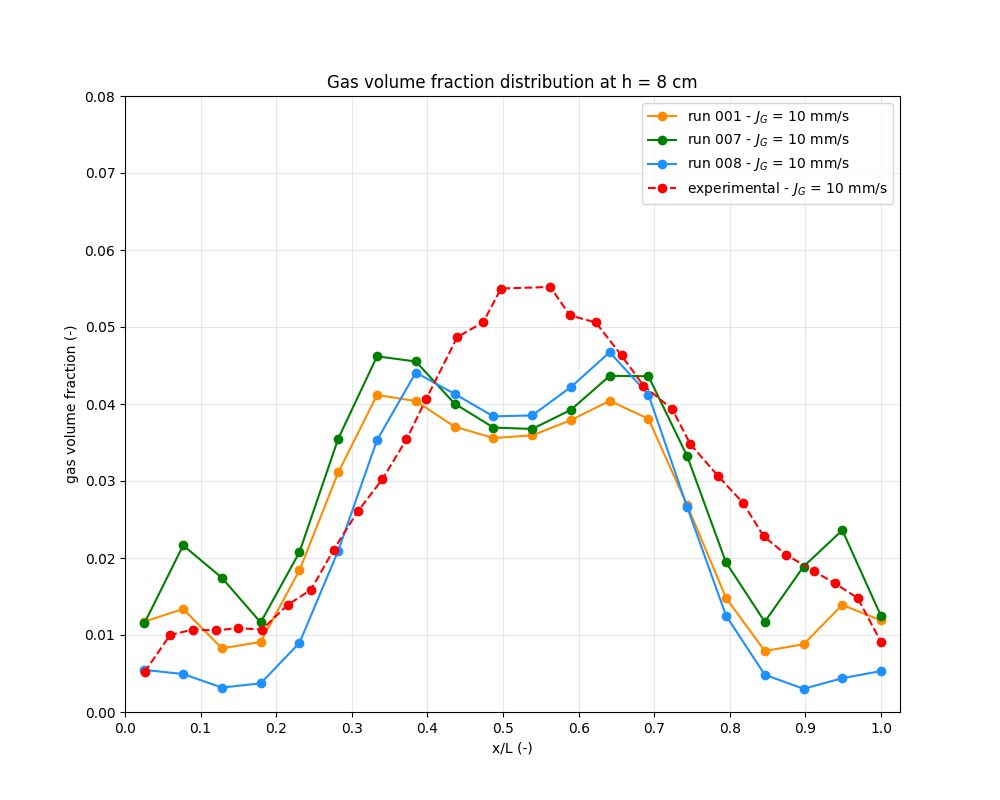
\includegraphics[scale=0.35]{Images/graphs/turbmodel/surfacesJ10h8.png}
    }
    \subfloat[h = 63 cm]{
        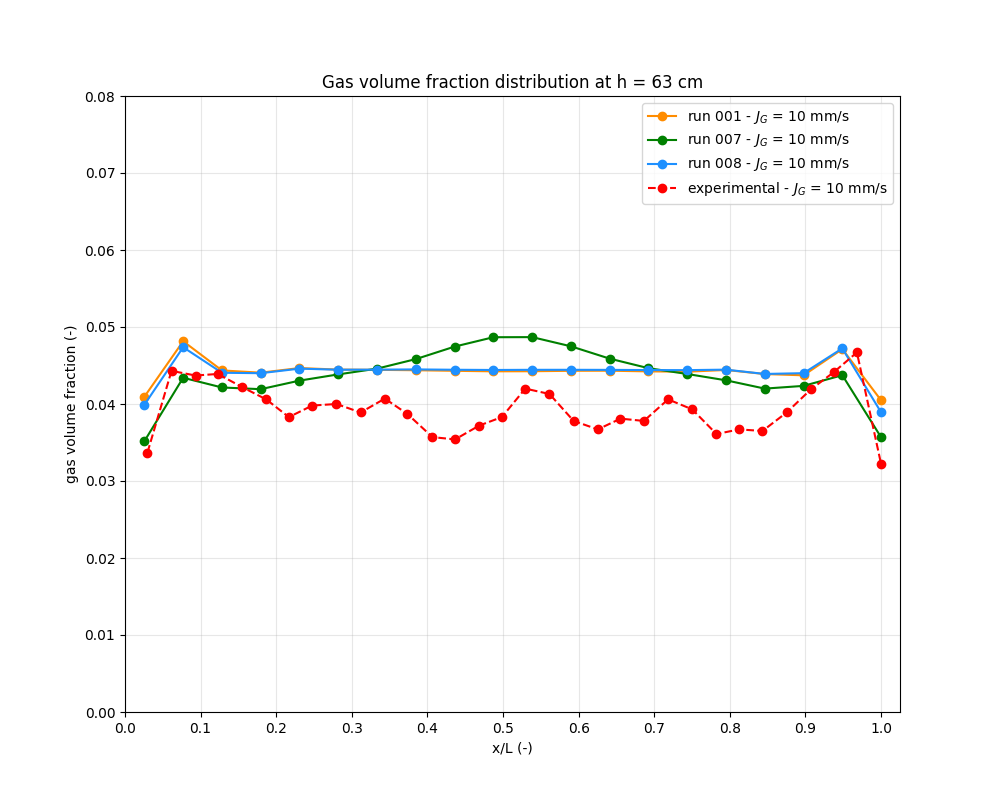
\includegraphics[scale=0.35]{Images/graphs/turbmodel/surfacesJ10h63.png}
    }
    \caption[]{Gas volume fraction horizontal distribution at different heights for different turbulence models}
    \label{fig:alpha_turbmodel}
\end{figure}

\subsection{Drag models}
\label{sub:drag_models}

\subsubsection{IshiiZuber}


\begin{table}[H]
    \centering 
    \begin{tabular}{|p{8em} c |}
    \hline
    \rowcolor{bluePoli!40}
    & \textbf{Drag model} \T\B \\
    \hline \hline
    \textbf{all runs} &  \T\B \\
    \hline
    \end{tabular}
    \\[10pt]
    \caption{Drag models}
    \label{table:drag_models}
\end{table}

\subsection{Lift models}
\label{sub:lift_models}

\subsubsection{Tomiyama}

\subsubsection{Moraga}

\begin{table}[H]
    \centering 
    \begin{tabular}{|p{8em} c |}
    \hline
    \rowcolor{bluePoli!40}
    & \textbf{Lift model} \T\B \\
    \hline \hline
    \textbf{run009} & None \T\B \\
    \textbf{run001} & Tomiyama \T\B \\
    \textbf{run010} & Moraga \T\B \\
    \hline
    \end{tabular}
    \\[10pt]
    \caption{Lift models}
    \label{table:lift_models}
\end{table}

\begin{figure}[H]
    \centering
    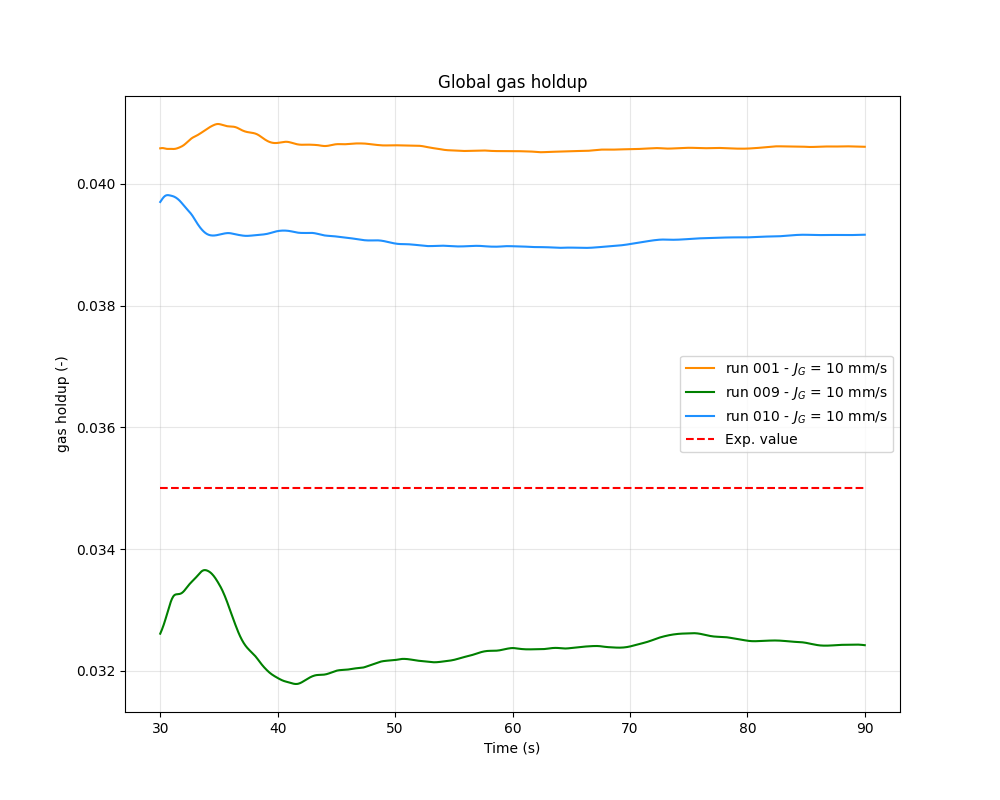
\includegraphics[width=0.5\textwidth]{Images/graphs/lift/holdUp10.png}
    \caption{Averaged holdup for different lift models}
    \label{fig:holdup_lift}
\end{figure}

\begin{figure}[H]
    \centering
    \subfloat[h = 8 cm]{
        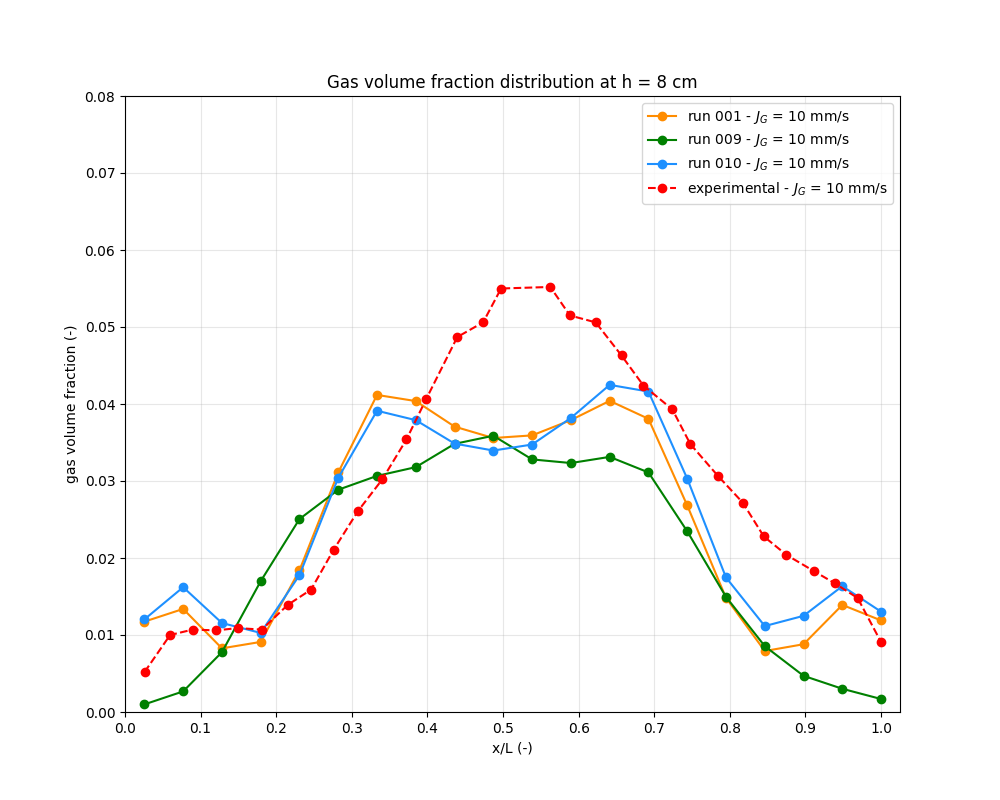
\includegraphics[scale=0.35]{Images/graphs/lift/surfacesJ10h8.png}
    }
    \subfloat[h = 63 cm]{
        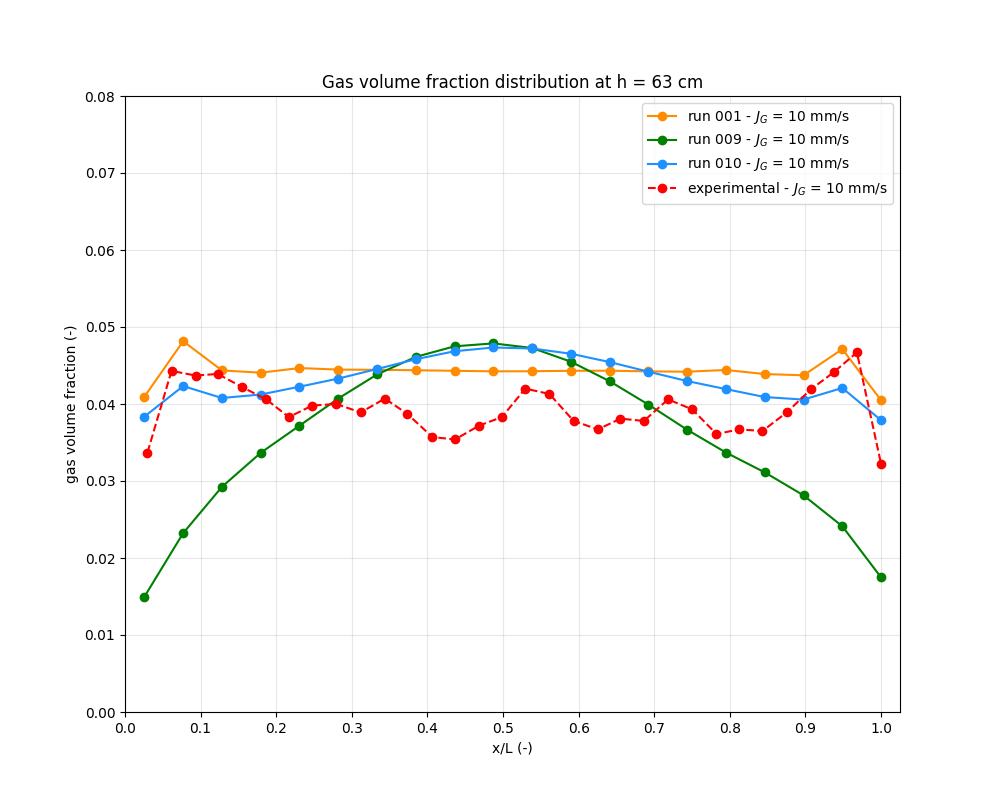
\includegraphics[scale=0.35]{Images/graphs/lift/surfacesJ10h63.png}
    }
    \caption[]{Gas volume fraction horizontal distribution at different heights for different lift models}
    \label{fig:alpha_lift}
\end{figure}

\subsection{Turbulent dispersion models}
\label{sub:turbulent_dispersion_models}

\subsubsection{Burns}

\subsubsection{LopezDeBertodanonone}

\begin{table}[H]
    \centering 
    \begin{tabular}{|p{8em} c |}
    \hline
    \rowcolor{bluePoli!40}
    & \textbf{Turbulent dispersion model} \T\B \\
    \hline \hline
    \textbf{run001} & None \T\B \\
    \textbf{run011} & Burns \T\B \\
    \textbf{run012} & LopezDeBertodanonone \T\B \\
    \hline
    \end{tabular}
    \\[10pt]
    \caption{Turbulent dispersion models}
    \label{table:turbulent_dispersion_models}
\end{table}

\begin{figure}[H]
    \centering
    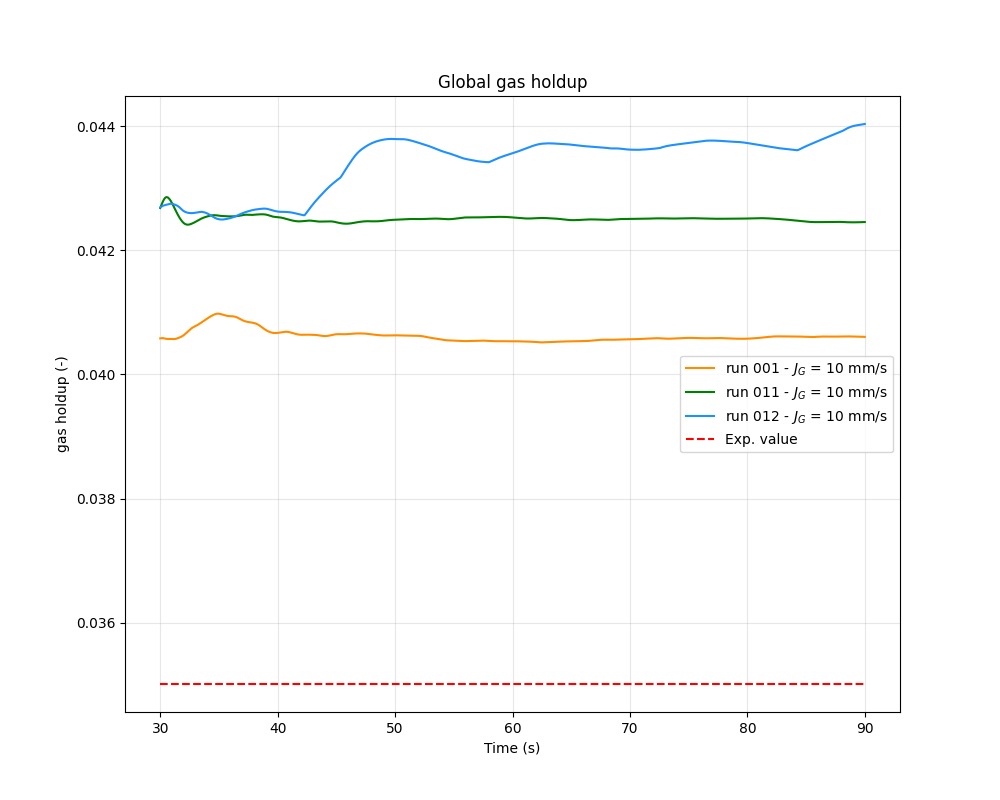
\includegraphics[width=0.5\textwidth]{Images/graphs/turbdisp/holdUp10.png}
    \caption{Averaged holdup for different turbulent dispersion models}
    \label{fig:holdup_turbdisp}
\end{figure}

\begin{figure}[H]
    \centering
    \subfloat[h = 8 cm]{
        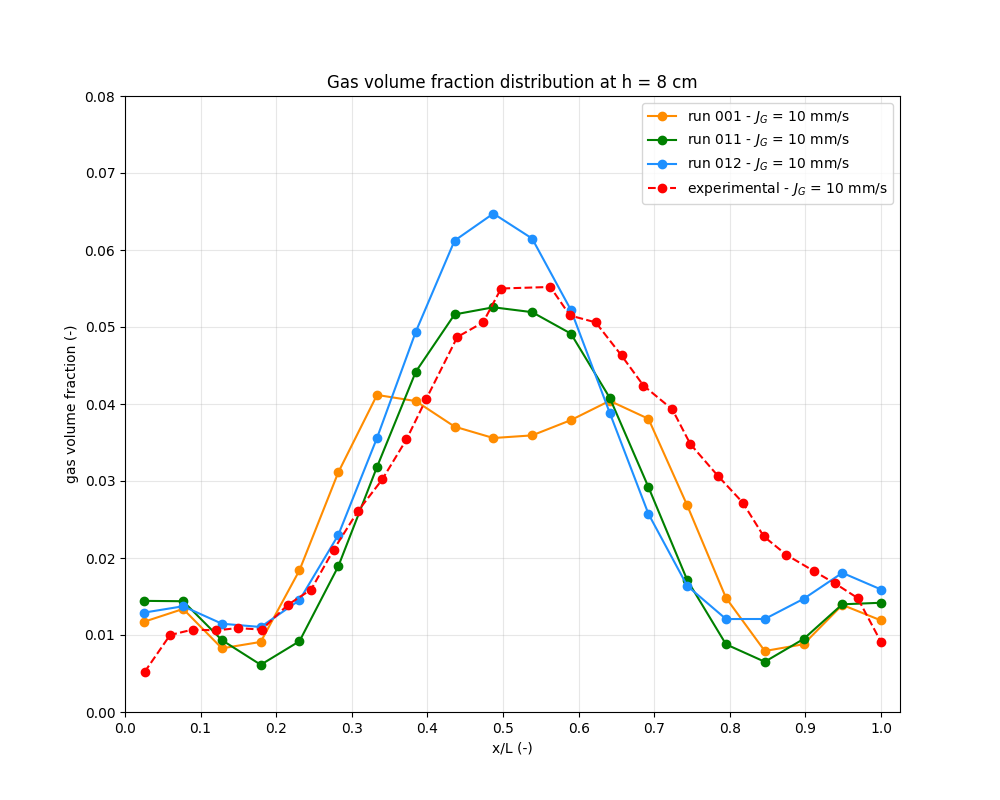
\includegraphics[scale=0.35]{Images/graphs/turbdisp/surfacesJ10h8.png}
    }
    \subfloat[h = 63 cm]{
        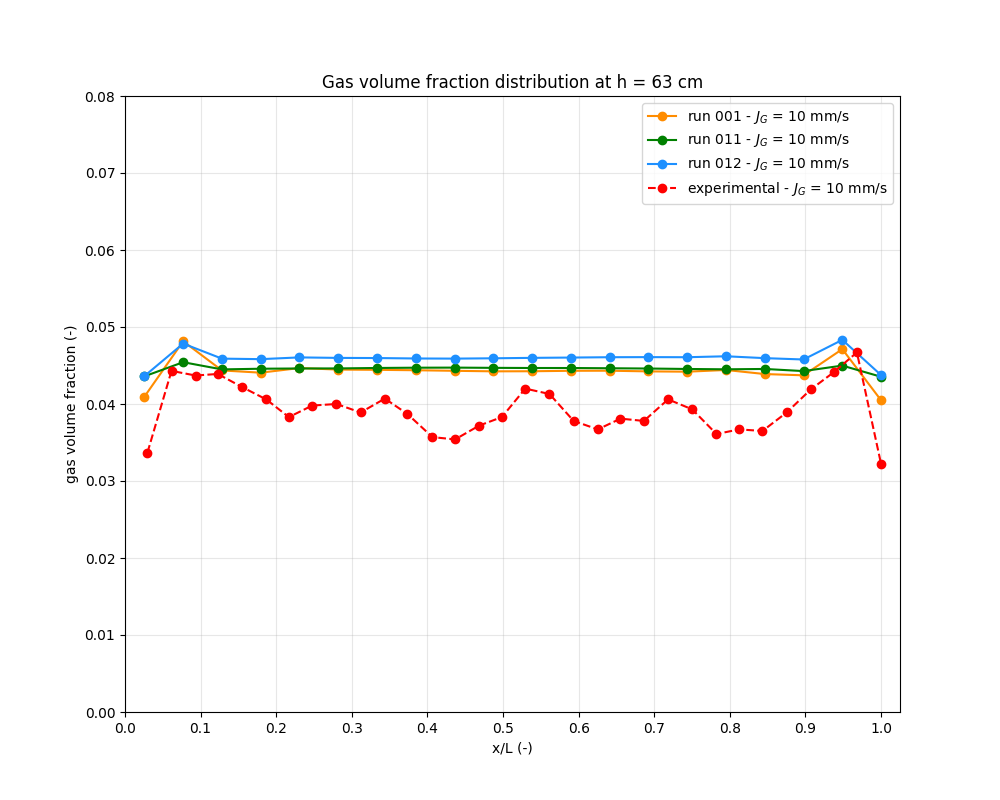
\includegraphics[scale=0.35]{Images/graphs/turbdisp/surfacesJ10h63.png}
    }
    \caption[]{Gas volume fraction horizontal distribution at different heights for different turbulent dispersion models}
    \label{fig:alpha_turbdisp}
\end{figure}

\subsection{Wall lubrication models}
\label{sub:wall_lubrication_models}

\subsubsection{Antal}

\subsubsection{Frank}

\begin{table}[H]
    \centering 
    \begin{tabular}{|p{8em} c |}
    \hline
    \rowcolor{bluePoli!40}
    & \textbf{Wall lubrication model} \T\B \\
    \hline \hline
    \textbf{run001} & None \T\B \\
    \textbf{run013} & Antal \T\B \\
    \textbf{run014} & Frank \T\B \\
    \hline
    \end{tabular}
    \\[10pt]
    \caption{Wall lubrication models}
    \label{table:wall_lubrication_models}
\end{table}

\begin{figure}[H]
    \centering
    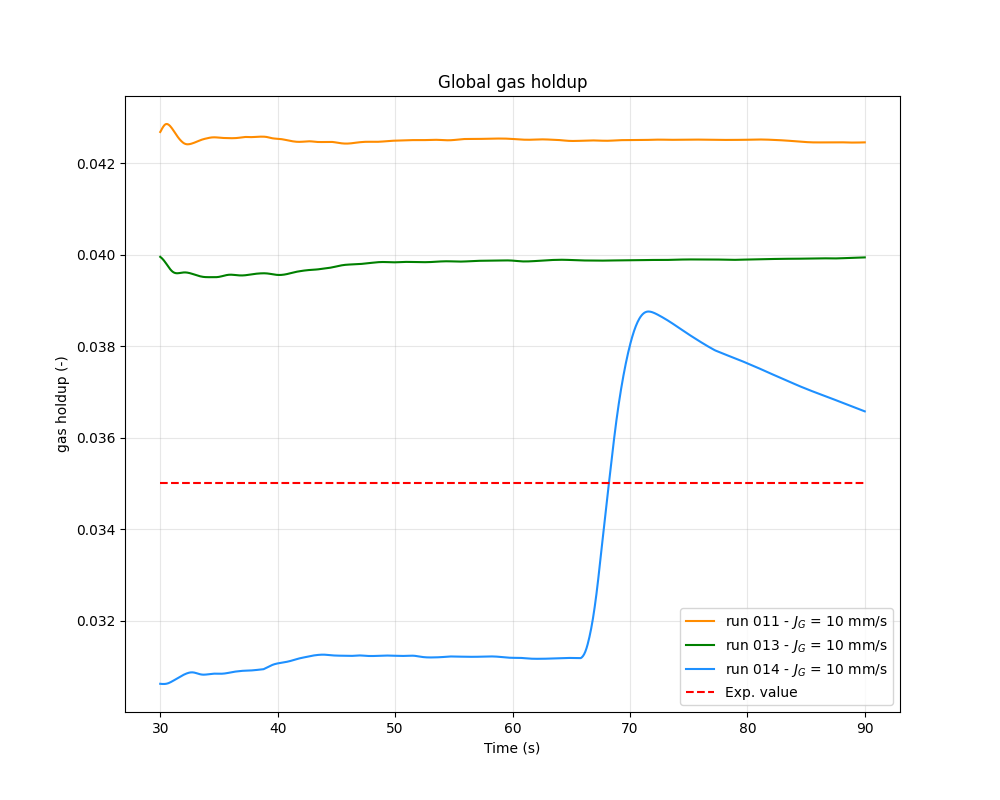
\includegraphics[width=0.5\textwidth]{Images/graphs/walllub/holdUp10.png}
    \caption{Averaged holdup for different wall lubrication models}
    \label{fig:holdup_walllub}
\end{figure}

\begin{figure}[H]
    \centering
    \subfloat[h = 8 cm]{
        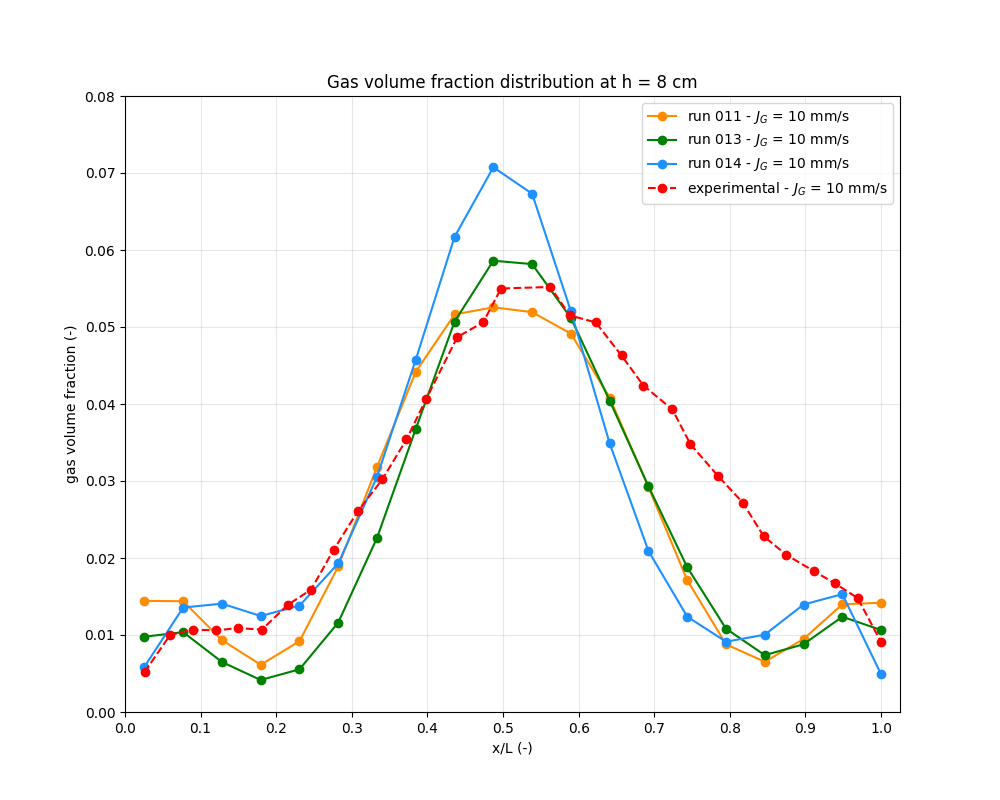
\includegraphics[scale=0.35]{Images/graphs/walllub/surfacesJ10h8.png}
    }
    \subfloat[h = 63 cm]{
        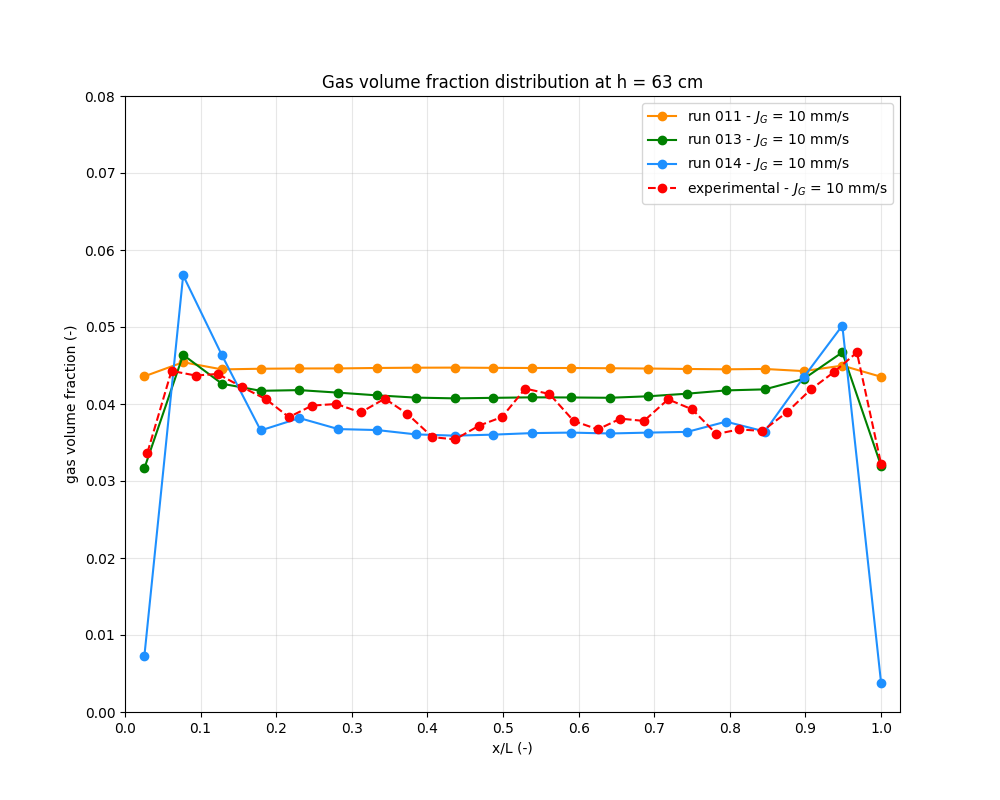
\includegraphics[scale=0.35]{Images/graphs/walllub/surfacesJ10h63.png}
    }
    \caption[]{Gas volume fraction horizontal distribution at different heights for different wall lubrication models}
    \label{fig:alpha_walllub}
\end{figure}

\subsection{Inflow velocity}
\label{sub:inflow_velocity}

\begin{table}[H]
    \centering 
    \begin{tabular}{|p{8em} c |}
    \hline
    \rowcolor{bluePoli!40}
    & \textbf{$J_{in} [mm/s]$} \T\B \\
    \hline \hline
    \textbf{run013} & 10  \T\B \\
    \textbf{run015} & 8  \T\B \\
    \textbf{run016} & 6 \T\B \\
    \hline
    \end{tabular}
    \\[10pt]
    \caption{Inflow velocities}
    \label{table:inflow_velocities}
\end{table}

\begin{figure}[H]
    \centering
    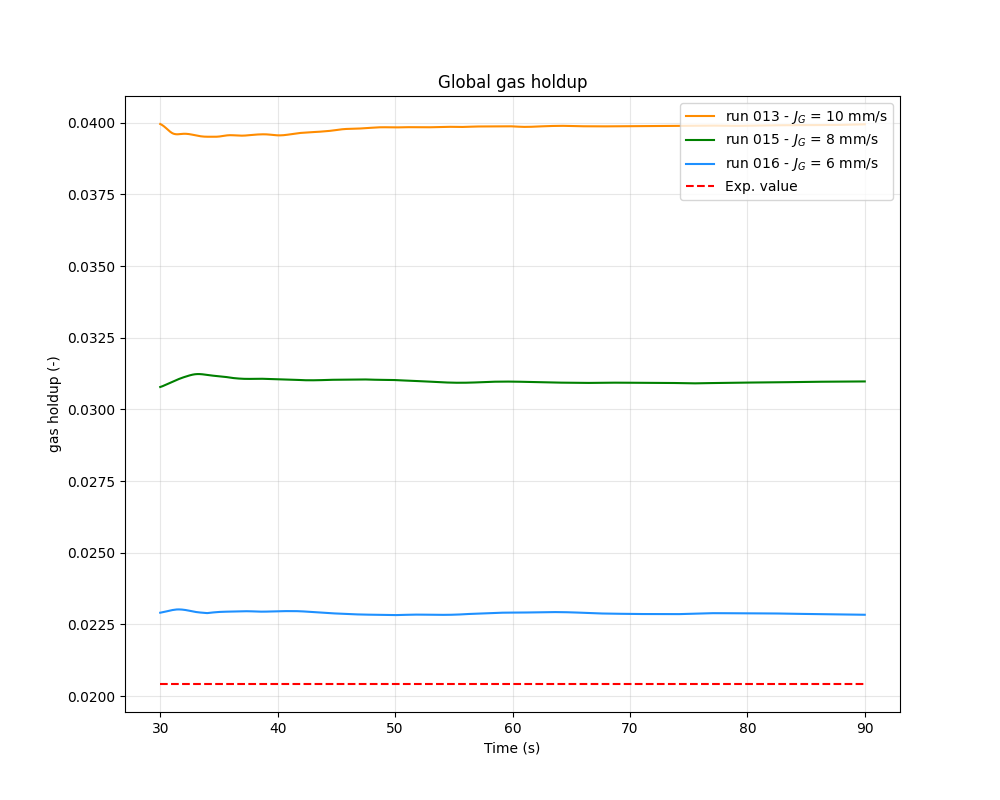
\includegraphics[width=0.5\textwidth]{Images/graphs/allj/holdUp6.png}
    \caption{Averaged holdup for different inflow velocities}
    \label{fig:holdup_inflow_velocities}
\end{figure}

\begin{figure}[H]
    \centering
    \subfloat[h = 8 cm]{
        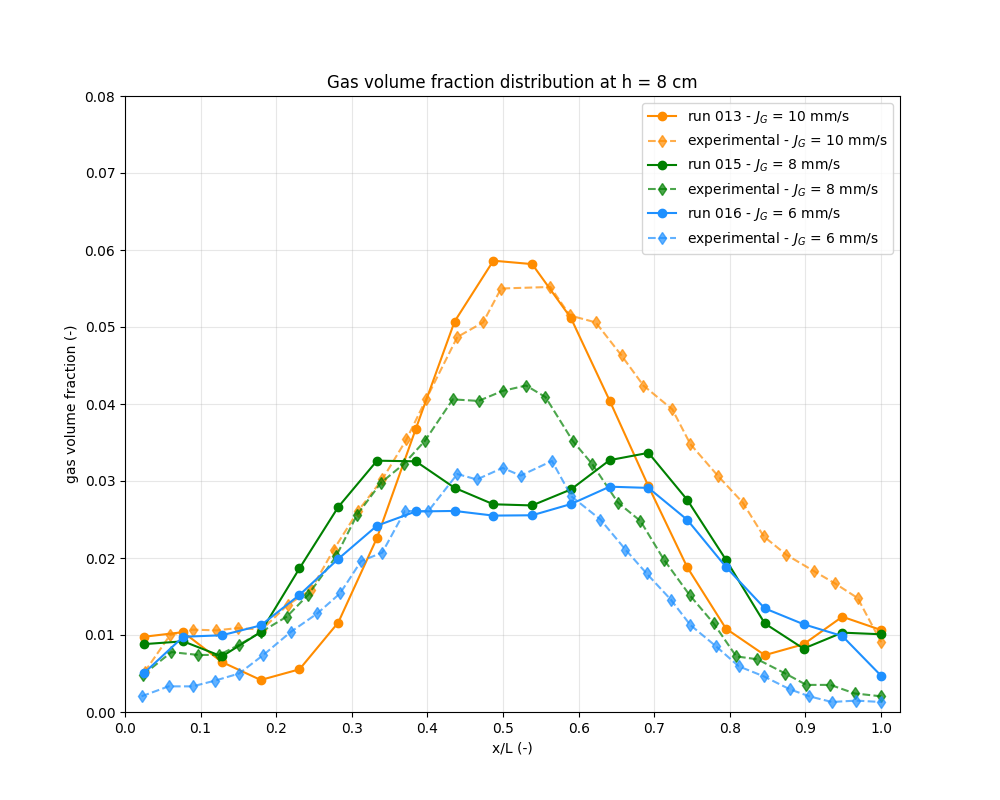
\includegraphics[scale=0.35]{Images/graphs/allj/surfacesJ6h8.png}
    }
    \subfloat[h = 63 cm]{
        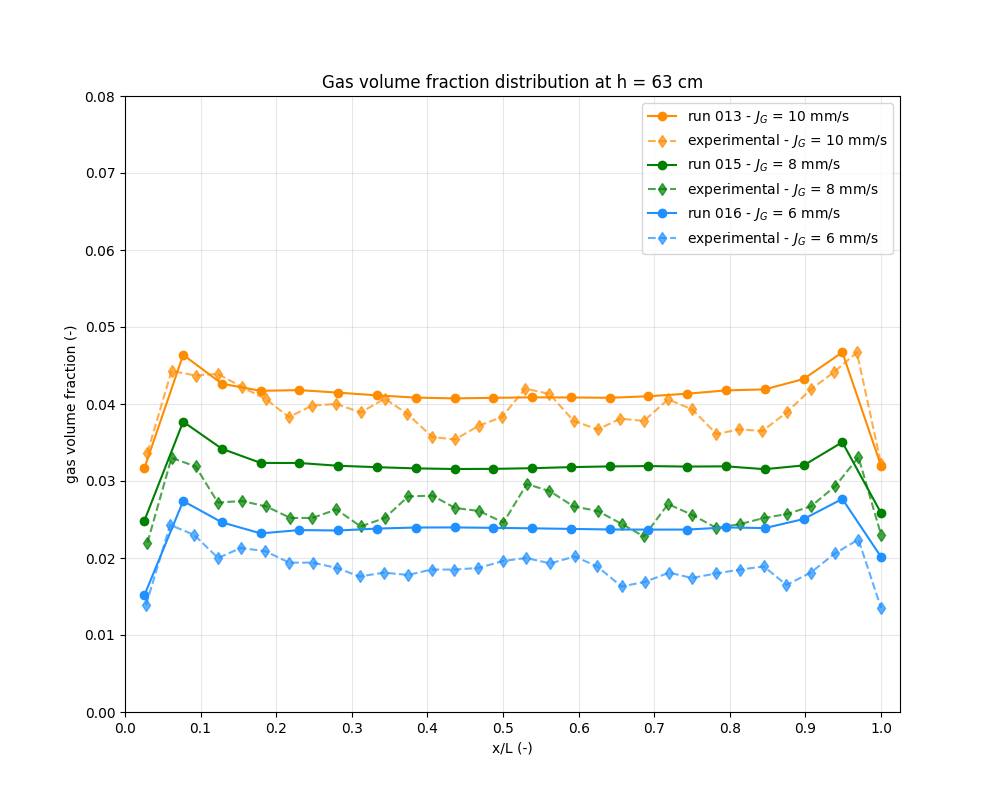
\includegraphics[scale=0.35]{Images/graphs/allj/surfacesJ6h63.png}
    }
    \caption[]{Gas volume fraction horizontal distribution at different heights for different inflow velocities}
    \label{fig:alpha_inflow_velocities}
\end{figure}

%-----------------------------------------------------------------------------
% BIBLIOGRAPHY
%-----------------------------------------------------------------------------
\bibliography{bibliography.bib}

\end{document}
